%%%%%%%%%%%%%%%%%%%%%%%%%%%%%%%%%%%%%%%%%
% University/School Laboratory Report
% LaTeX Template
% Version 3.1 (25/3/14)
%
% This template has been downloaded from:
% http://www.LaTeXTemplates.com
%
% Original author:
% Linux and Unix Users Group at Virginia Tech Wiki 
% (https://vtluug.org/wiki/Example_LaTeX_chem_lab_report)
%
% License:
% CC BY-NC-SA 3.0 (http://creativecommons.org/licenses/by-nc-sa/3.0/)
%
%%%%%%%%%%%%%%%%%%%%%%%%%%%%%%%%%%%%%%%%%

%----------------------------------------------------------------------------------------
%	PACKAGES AND DOCUMENT CONFIGURATIONS
%----------------------------------------------------------------------------------------

\documentclass{article}

\usepackage[version=3]{mhchem} % Package for chemical equation typesetting
\usepackage{siunitx} % Provides the \SI{}{} and \si{} command for typesetting SI units
\usepackage{graphicx, xcolor} % Required for the inclusion of images
\usepackage{natbib} % Required to change bibliography style to APA
\usepackage{amsfonts}
\usepackage{amssymb}
\usepackage{amsmath} % Required for some math elements 
\usepackage{svg} % .svg support
\usepackage[nolist]{acronym}
\usepackage{trfsigns}


\usepackage{minted}
\definecolor{bg}{rgb}{0.95,0.95,0.95}

\graphicspath{{img/}}

\setlength\parindent{0pt} % Removes all indentation from paragraphs

\renewcommand{\labelenumi}{\alph{enumi}.} % Make numbering in the enumerate environment by letter rather than number (e.g. section 6)

%\usepackage{times} % Uncomment to use the Times New Roman font

%----------------------------------------------------------------------------------------
%	DOCUMENT INFORMATION
%----------------------------------------------------------------------------------------

\title{Projekt: Mobilfunk und Signalverarbeitung} % Title

\author{Lukas Becker, Tobias Frahm} % Author name

\date{\today} % Date for the report

\begin{document}

\maketitle % Insert the title, author and date

\begin{center}
\begin{tabular}{l r}
Date Performed: & \today \\ % Date the experiment was performed
Partners: & Lukas Becker, Tobias Frahm \\ % Partner names
Instructor: & Prof. Dr. Sauvagerd \\% Instructor/supervisor
University: & University of Applied Science 
\end{tabular}
\end{center}

\begin{acronym}
    \acro{CPFSK}{Continous Phase Frequency Shift Keying}
\end{acronym}

% If you wish to include an abstract, uncomment the lines below
% \begin{abstract}
% Abstract text
% \end{abstract}

%----------------------------------------------------------------------------------------
%	SECTION 1
%----------------------------------------------------------------------------------------

\section{Projektbeschreibung und Ziel des Projektes}

In diesem Projekt wird eine \ac{CPFSK} Demodulation und Dekodierung eines Wetterberichtes über Kurzwelle 
(Seewetterbericht des  Senders  Pinneberg  auf  Kurzwelle)  in  Echtzeit  durchgeführt. 
Diese  \ac{CPFSK} Demodulation  wird  in  Form  eines  \textit{Software  Radios}  auf  einem  
Digitalen Signalprozessor (DSP) implementiert. 

Das \ac{CPFSK}-modulierte Kurzwellensignal wird mit einer Draht-Antenne im Frequenzbereich
$10.1Mhz$ bis $11.1MHz$ empfangen und verstärkt. Die Daten werden hierbei mithilfe des Baudot-Codes kodiert. Ziel das Projektes ist es, zunächst in \textit{MATLAB} ein Modell zu erstellen, welches
in der Lage ist, die \ac{CPFSK} modulierten Seewetterdaten zu demodulieren und dekodieren sowie das Ergebnis in Form eines $string$ auszugeben. 
Für das \textit{MATLAB} Modell wird hierfür zunächst ein \ac{CPFSK}-moduliertes Signal in \textit{MATLAB} erzeugt um die ersten 
Schritte durchzuführen. Zur Überprüfung der Anwendbarkeit wird im Folgenden auf ein aufgenommenes Signal zurückgegriffen.
Sobald das \textit{MATLAB} Modell steht, wird die Simulation in C-Code überführt und anschließend 
auf einem DSP implementiert. Geschuldet der aktuellen Situation im Bezug auf den Ausbruch von COVID-19 konnte ein realer Test auf dem DSP nicht durchgeführt werden. 

\section{Vorbereitung}
Um ein grundlegendes Verständnis für das Projekt zu bekommen, werden zunächst einige Ansätze in \textit{MATLAB} simuliert.
Hierfür wird zuächst eine Rechteckfolge mit dem Wertebereich $D = \{-1,1\}$ generiert. Anschließend wird die Anfangsphase für das CPFSK Signal bestimmt. Diese wird genutzt um zunächst ein 
\ac{CPFSK} moduliertes Testsignal zu erzeugen. Mit dem so erzeugtem CPFSK Signal, kann eine erste Bandbreitenabschätzung durchgeführt werden.


\subsection{Rechteckimpuls $d(i)$ - Worksheet01}\label{sec:rechteck}
Mit Angabe der Symboldauer $T = 20ms$ lässt sich auf die minimale Abtastfrequenz nach Nyquist-Shannon schließen.
Die minimale Abtastfrequenz $f_A$ muss mehr als doppelt so groß wie die höchste abzutastende Frequenz sein.

Aus
\begin{center}
 $
f_A > 2*f_{max}
$
\end{center}

mit 
\begin{center} $f_{max} = \frac{1}{T_{max}} ; T_{max} = T = 20ms$  \end{center}

ergibt sich

\begin{center}
$
f_A > 2*\frac{1}{T}
$
\end{center}

Eingesetzt:
\begin{center}
$f_A > 2*\frac{1}{20ms}$
\end{center}
\begin{center}
$f_A > 100Hz$   
\end{center}
\begin{figure}[!h]
    \centering
    \def\svgscale{0.3}
    \def\svgwidth{\columnwidth}
    \input{img/rechteck.pdf_tex}
    \caption{Rechteckimpuls zur \ac{CPFSK} Simulation in \textit{MATLAB}}
\end{figure}

\subsection{Anfangsphase $\phi(iT)$ - Worksheet01}
Für die \ac{CPFSK}-Modulation muss die Anfangsphase $\phi(iT)$ bestimmt werden.
Gegeben ist ein Integrator (IIR Filter 1.Ordnung) mit der Übertragungsfunktion:
$$
H_I(z)=\frac{z^{-1}}{1-z^{-1}}
$$
Dieser kann hier anstelle der Summenbildung der komplexen Einhüllenden eingesetzt werden, 
da die Integration einer Aufsummierung diskreter Flächenelemte unter der Kurve entspricht.

\begin{figure}[!h]
    \centering
    \def\svgscale{0.3}
    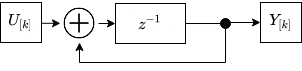
\includegraphics{img/sig_IIR.png}
    \caption{Signalflussdiagramm des Integrators 1.Ordnung}
\end{figure}

\subsection{\ac{CPFSK} Signal - Worksheet01}

Die \ac{CPFSK} Modulation ist eine Methode um digitale Signale mithilfe einer Trägerfrequenz analog zu Übertragen.
Bei der \ac{CPFSK} Modulation handelt es sich um eine Frequenzmodulation ohne Sprünge im Phasenübergang. In Abb.~\ref{fsk}
ist im oberen Bereich das binäre Signale, im mittleren Bild die Trägerfrequenz und unten das binäre Signal auf die Trägerfrequenze
moduliert zu sehen. Der Phasenübergang ohne Sprung ist notwendig, da Sprünge ein theoretisch unendliches breites Band benötigen
somit die Nachbarkanäle stören würde.
\begin{figure}[!h]
    \centering

    \def\svgwidth{0.6\columnwidth}
    \input{img/fsk.pdf_tex}
    \caption{Beispielhaftes \ac{CPFSK} moduliertes Trägersignal einer binären 
    Information. Die Phasenübergänge sind ohne Sprung. }%´Quelle:~\cite{wiki:fsk}}
    \label{fsk}
\end{figure}

Das in Abschnitt~\ref{sec:rechteck} generierte Rechtecksignal wird nun \ac{CPFSK} moduliert.
Dafür wir die Formel aus Worksheet 1 verwendet:

$$CPFSK_{sig} = amp \cdot  sin(2  \pi \cdot f_T \cdot n \cdot T_A + 2 \pi \cdot \varDelta{F} \cdot \frac{\phi (iT)}{f_A} + \varphi_0) $$

Zur bestimmung des Spektrums des Signals, wird in \textit{MATLAB} die FFT verwendet.
\begin{figure}[!h]
    \centering
    \def\svgscale{0.3}
    \def\svgwidth{\columnwidth}
    \input{img/spektrum.pdf_tex}
    \caption{Betragspektrum des \ac{CPFSK}-Modulierten Rechteckimpulses.}
\end{figure}
Bei einem $\varDelta F = 225Hz$ wird hier eine Bandbreite von ca. $B > 450Hz = 2\cdot \varDelta F $ erwartet.

Zur Bandbreitenbestimmung wird das Parsevalsche Theorem genutzt, die Bandbreite des \ac{CPFSK} Signals ist derjenige Bereich,
in den 99\% der Signalenergie von $0...\frac{f_A}{2}$ Fallen. Es ergibt sich hierbei eine Bandbreite von $704Hz$

$$
\sum_{n = 0}^{N - 1}\left\lvert x(n)^2\right\rvert =  \frac{1}{N} \sum_{k = 1}^{N-1}  \left\lvert X(k)^2\right\rvert 
$$
\begin{listing}
\begin{minted}[linenos, bgcolor=bg, breaklines]{matlab}
% Die Bandbreite wird durch den Breich beschrieben, in den 99%
% der Signalenergie fallen.

total_power = 0;
current_power = 0;
idx = 0;
idx_max = round(length(spectrum_sig)/2);
idx_start = idx_max/2; % fA/4

for i = 1:length(spectrum_sig)/2 - 1
    total_power = total_power + abs(spectrum_sig(i))^2 / length(spectrum_sig);
end

N = length(spectrum_sig);

while current_power/total_power < 0.99
    current_power = current_power + abs(spectrum_sig(idx_start - idx))^2 / N;
    current_power = current_power + abs(spectrum_sig(idx_start + idx))^2 / N;
    idx = idx + 1;
end
\end{minted}
\end{listing}

Das Weglassen der Start- und Stopbits spielt bei der Bestimmung der Bandbreite keine rolle.
Es werden nur binäre Daten übertragen $D = \{0, 1\}$. die Frequenzen $ f_{0, 1} = f_T \pm \varDelta F $ repräsentieren. 
Da auch die Start/Stopbits durch $D$ dargestellt werden, würde sich hier im Frequenzbereich
nur eine Veränderung im Maximum der Amplitude ergeben, die repräsentierenden Frequenzen selbst bleiben unverändert.

\subsection{FM Verzögerungsdemodulator - Worksheet02}

\begin{figure}[!h]
    \centering
    \def\svgscale{0.5}
    \def\svgwidth{\columnwidth}
    \input{img/ws02_fluss.pdf_tex}
    \caption{FM Basisband-Verzögerungsdemodulator. Quelle: Worksheet02}
    \label{fig:fm-verz}
\end{figure}

Zur demodulation des Signals soll ein FM Verzögerungsdemodulator zum Einsatz kommen. Dieser ist für die Symbolrückgewinnung zuständig. 
Das Eingangssignal des Signalflussdiagramm in Abb.~\ref{fig:fm-verz} wird in dem Worksheet wie folgt beschrieben:

$$
v(n) = v e^{j w_0 n}
$$

Der Zusammenhang zwischen $v(n)$ und dem Ausgangsignal $y(n)$ ergibt sich hier wie folgt:

$$
y(n) = v e^{j w_0 n} \cdot v e^{-j w_0 (n-1)} = v^2 e^{j w_0}
$$

weiterhin ergibt sich für $y_{CPFSK}(n)$ und $v(n)$:

$$
y_{CPFSK}(n) = \Im(v(n) v^\ast(n-1)) = \Im( v^2 e^{j w_0}) = \Im(v^2 (sin(w_0) + j cos(w_0)))
$$

$$
y_{CPFSK}(n) = v^2 \cdot sin(w_0)
$$

Um die Frequenz am Ausgang zu bestimmen, muss nach $w_0$ umgestellt werden und der $arcsin()$ angewand werden:

$$
sin(w_0) = \frac{y_{CPFSK}(n)}{v^2}
$$

$$
w_0 = arcsin(\frac{y_{CPFSK}(n)}{v^2})
$$

Das in Abb.~\ref{fig:fm-verz} zu sehende Signalflussdiagramm gilt für den Wertebereich:
$$
-1 \leq  \frac{y_{CPFSK}(n)}{v^2} \leq 1
$$

Um die Begrenzung durch den Wertebereich zu Verhindern, muss, wie in Abb.~\ref{fig:signal} zu sehen, 
das Eingangssignal mit dem Faktor $\frac{1}{v}$ Verstärkt werden.

In Teilaufgabe 2 des Worksheets soll nun das Signalflussdiagramm in Matlab umgesetzt werden.
Dafür wurde zunächst das in Abb.~\ref{fig:cpfsk} gezeigte CPFSK Signal in \textit{MATLAB} erzeugt.


\begin{figure}[!h]
    \centering
    \def\svgscale{0.5}
    \def\svgwidth{0.8\columnwidth}
    \input{img/cpfsk.pdf_tex}
    \caption{CPFSK Signal: Man erkennt deutlich die Wechsel der Mark/Space Frequenzen.}
    \label{fig:cpfsk}
\end{figure}

Um das reele Signal dem FM-Demodulator übergeben zu können, wird es durch einen Hilbert-Transformator gefiltert.
Dies ist in der \textit{MATLAB} Simulation in listing.~\ref{codeM:hilbert} gezeigt. Die  Abb.~\ref{fig:hilbert_vor} und Abb.~\ref{fig:hilbert_nach} zeigen das Signal vor und nach 
der Anwendung des Hilbert Filters. Das reele Signal wird zu einem koplexen Signal.

\begin{figure}[!h]
    \centering
    \def\svgscale{0.5}
    \def\svgwidth{0.8\columnwidth}
    \input{img/hil_vor.pdf_tex}
    \caption{Amplitudengang des reelen Signals}
    \label{fig:hilbert_vor}
\end{figure}

\begin{figure}[!h]
    \centering
    \def\svgscale{0.5}
    \def\svgwidth{0.8\columnwidth}
    \input{img/hil_nach.pdf_tex}
    \caption{Amplitudengang des komplexen Signals}
    \label{fig:hilbert_nach}
\end{figure}

\begin{listing}\label{codeM:hilbert}
    \caption{CPFSK Signal Hilbert gefiltert, jeweils für die Mark und Space Frequenzen}
    \begin{minted}[linenos, bgcolor=bg, breaklines]{matlab}
v_max = 0.5;
fA = 4000;
n = 1:1:fA;
fT = fA/4;
fHub = 225;
fSpace = fT - fHub;
fMark = fT + fHub;
sqre = out;
phi_0 = pi;
num_integrator = [0, 1];
den_integrator = [1, -1];

Phi_iT = filter(num_integrator, den_integrator, sqre(1:801)) + phi_0;
cpfsk_sig = v_max * sin(2 * pi * fT * n(1:801)/fA + 2 * fHub * pi * Phi_iT/fA + phi_0);
fn = (-length(n(1:801))/2:(length(n(1:801))-1)/2) * fA/length(n(1:801));

plot(n(1:801), cpfsk_sig)
xlim([0, 400])
title('CPFSK Moduliertes Signal')
xlabel(['Samples [n]'])
ylabel(['Amplitude'])

plot(fn, abs(fft(cpfsk_sig)))
title('CPFSK Moduliertes Signal (vor Hilbert Transformation)')
xlabel(['Frequenz [Hz]'])
ylabel(['Amplitude'])
grid on;


Phi_iT1 = filter(num_integrator, den_integrator, sqre(1:82)) + phi_0;
cpfsk_sig1 = v_max * sin(2 * pi * fT * n(1:82)/fA + 2 * fHub * pi * Phi_iT1/fA + phi_0);
y1 = hilbert(cpfsk_sig1);

Phi_iT0 = filter(num_integrator, den_integrator, sqre(83:162)) + phi_0;
cpfsk_sig0 = v_max * sin(2 * pi * fT * n(83:162)/fA + 2 * fHub * pi * Phi_iT0/fA + phi_0);
y0 = hilbert(cpfsk_sig0);

fn0 = (-length(n(1:82))/2:(length(n(1:82))-1)/2) * fA/length(n(1:82));
plot(fn0, abs(fftshift(fft(y1))/length(n(1:82))))
hold on;
fn1 = (-length(n(83:162))/2:(length(n(83:162))-1)/2) * fA/length(n(83:162));
plot(fn1, abs(fftshift(fft(y0))/length(n(83:162))))

title('CPFSK Spektren (nach Hilbert Transformation)')
xlabel(['Frequenz [Hz]'])
ylabel(['Amplitude'])
    \end{minted}
\end{listing}


\section{Signalfluss Empfänger}

Abb.~\ref{fig:signal} zeigt den Aufbau des Softwareradios. Das durch ein analoges Bandpassfilter extrahierte, zwischen $10.1Mhz$ und $11.1Mhz$ befindliche Band wird empfangen, und durch Unterabtastung mithilfe des ADCs in das auf das Band bezogene Basisband verschoben.
Hierbei wird das Band auf $1.0096Mhz$ Nyquistbandbreite geschmälert. Ein Dezimator mit Bandpass als Anti-Aliasingfilter (Kapitel~\ref{sec:FIR}) reduziert die Abtastfrequenz auf $3831,49Hz$. Der Durchlassbereich des Bandpasses wird hierbei jeweils auf den zu empfangenden Kanal angepasst. Die beiden Frequenzen für Mark (-1) und Space (-1) befinden sich im Basisband. Zur Symbolrückgewinnung durch Demodulation können unterschiedliche Methoden der Vorverarbeitung angewandt werden, in dieser Arbeit wurde zunächst ein Ansatz über einen Hilberttransformator, Kapitel~\ref{sec:hilbert} verfolgt. Im laufe des Projektes hat sich jedoch die Verwendung eines komplexen Kammfilters
als stabilere Alternative herausgestellt. Das Kammfilter in Kapitel~\ref{sec:comb} sorgt dafür, dass die Frequenzen deutlich von einander zu differenzieren sind. Sobald das Signal durch das Kammfilter
aufbereitet ist, kann die Demodulation durch einen FM-Verzögerungsdemodulator \ref{sec:fm-demod} mit anschließender Dekodierung erfolgen.


\begin{figure}[!h]
    \centering
    \def\svgscale{0.5}
    \def\svgwidth{\columnwidth}
    \input{img/signal.pdf_tex}
    \caption{Durch den ADC findet direkt beim Empfang eine Unterabtastung statt. Durch eine weitere Unterabtastung im Bandpass, wird das Signal in das Basisband verschoben.
    Anschließen durch das Kammfilter für die Demodulation mit anschließender Dekodierung aufbereitet und auf dem Hyperterminal angezeigt.}
    \label{fig:signal}
\end{figure}

\section{Dezimator mit Kanalselektion}\label{sec:FIR}
Der Wetterdatensender sendet auf mehreren Kanälen in dem genannten Band. Nun muss der jeweils ein Kanal mithilfe eines Bandpasses selektiert werden. Der so ausgewählte Kanal wird nun mithilfe einer Unterabtastung in den Tiefpassbereich verschoben um eine Demodulation durchführen zu können. Zur Steigerung der Recheneffizienz wird eine Dezimationsstufe realisiert, die im Unterabtaster direkt mit den Polyphasen des Bandpasses filtert. So werden pro empfangenen Sample nur sehr wenige Multiplikationen durchgeführt. Das Filter wird in \textit{MATLAB} ausgelegt und dann in Polyphasen zerlegt exportiert. Die exportierte Datei kann direkt als Feld in C verwendet werden.

\subsection{Theorie}
Der bei 10100.8 kHz befindliche, 5KHz breite Kanal wird durch die Unterabtastung in den 
Bereich von 4800Hz +/- 2500Hz verschoben. 
Da sich im schlechtesten Fall direkt daneben der nächste Kanal anschließt, muss vor einer Unterabtastung gefiltert werden um Aliasing zu vermeiden. 
Der Filter muss nun einen Durchlassbereich von mindestens der 99\% Bandbreite bzw. $704Hz$ aufweisen, maximal 
jedoch einen Durchlassbereich von $5Khz$ weniger zwei mal dem Übergangsbereich, um zuverlässig danebenliegende Bänder zu dämpfen. 
Die Grenzen des Durchlassbereiches werden somit auf $f_u = 3800Hz$ und $f_o = 4800Hz$ festgelegt, der Übergangsbereich auf jeweils 1500 Hz um die
Anzahl der Koeffizienten gering zu halten. Zudem wird der Bandpass als FIR-Filter realisiert. Der nachfolgende Unterabtaster 
wird mit dem Faktor 527 betrieben, woraus sich eine Abtastfrequenz von $f_{s_{neu}} = 3831,499Hz$ ergibt. Somit verteilen sich die 
2056 Koeffizienten des Filters auf 527 Polyphasen mit jeweils vier Koeffizienten. Da nicht jede der Polyphasen vier Koeffizienten aufweisen kann, 
werden Nullen eingefügt.

\subsection{MATLAB}
Zu Auslegung des FIR Filters in \textit{MATLAB} listing~\ref{codeM:FIRBP}, müssen zunächst die Grenz- und Stopfrequenzen Festgelegt werden.
Es ergeben sich $f_u = 3800Hz$ und $f_o = 4800Hz$, die Stopfrequenzen $f_{uStop} = f_u - 1500$ und $f_{oStop} = f_o + 1500$.
Bei den Stopfrequenzen gilt es Abzuwägen: Umso steiler das Filter, desto mehr Koeffizienten, desto mehr Rechenzeit wird später in C
benötigt. Der Amplitudengang des Filters, siehe Abb.~\ref{fig:fir_ampli}, zeigt das gewünschte Verhalten. Es werden $2056$ Koeffizienten benötigt.

\begin{figure}[!h]
    \label{fig:fir_ampli}
    \centering
    \def\svgscale{0.3}
    \def\svgwidth{\columnwidth}
    \input{img/FIR_BP.pdf_tex}
    \caption{FIR-Bandpassfilter Amplitudengang. Das FIR Filter benötigt 2056 Koeffizienten.}
\end{figure}
\begin{listing}\label{codeM:FIRBP}
    \caption{FIR-Bandpass Filterfunktion in \textit{MATLAB}}
    \begin{minted}[linenos, bgcolor=bg, breaklines]{c}
function [outputArg1, outputArg2, outputArg3] = band(low, high, inputSig, sample_rate)
%FIR Bandpass
%
rp = 3; 
rs = 40;
dev = [(10^(rp/20)-1)/(10^(rp/20)+1) 10^(-rs/20)]; 
low_stop = low - 1500;
high_stop = high + 1500;
[N_FIR,fo,mo,w] = firpmord([low_stop low high high_stop], [0 1 0], [0.05, 0.01, 0.05], sample_rate);
fprintf("N_FIR = %d\n", N_FIR);
coeff = firpm(N_FIR,fo,mo,w);

freqz(coeff,1, 200000, sample_rate)

xb = filter(coeff, 1, inputSig);
outputArg1 = xb;
outputArg2 = coeff;
outputArg3 = fo;
end
    \end{minted}
\end{listing}
\subsection{ANSI C}
Der Dezimator wird als Zähler realisiert (vgl. \ref{codeC:dezimation}), der bei Überlauf die Summe aller gefilterten Polyphasen berechnet und diese zur weiteren Verarbeitung zwischenspeichert. Die Filterkoeffizienten werden aus Effizienzgründen als \textit{const short} ausgeführt. Festkommaarithmetik sowie Zugriffe auf im ROM angelegte Variablen des Typs \textit{const} sind hierbei entscheidende Optimierungen.
Die Datenstruktur enthält hierbei 527 Felder mit jeweils vier Werten, also jeweils 64Bit. Dieser werden per Referenz der Filterroutine übergeben. Es wird Abtastwert für Abtastwert eingelesen, dezimiert und durch die Filterroutine verarbeitet lst.~\ref{codeC:FIR}.
\begin{listing}\label{codeC:dezimation}
    \caption{Beispielhafte Polyphase in C, die Koeffizienten sind im Datentyp \textit{short} abgelegt.}
    \begin{minted}[linenos, bgcolor=bg]{c}
const short FIR_BANDPASS_1[4] = {1304, 22, 186, -8,};
    \end{minted}
\end{listing}
\begin{listing}\label{codeC:FIR}
    \caption{FIR-Polyphasenbandpass Implementierung in C}
    \begin{minted}[linenos, bgcolor=bg, breaklines]{c}
short FIR_filter_sc(short FIR_delays[], const short FIR_coe[], short int N_delays, short x_n, int shift) {
    short i, y;
    int FIR_accu32 = 0;
    // read input sample from ADC
    FIR_delays[N_delays-1] = x_n;	 
    // clear accu
    FIR_accu32	= 0;
    // FIR filter routine				
    for( i = 0 ; i < N_delays ; i++ )		
        FIR_accu32 += FIR_delays[N_delays-1-i] * FIR_coe[i];
    
    for( i = 1 ; i < N_delays ; i++ )				
        FIR_delays[i-1] = FIR_delays[i];

    y = (short) (FIR_accu32 >> shift);
    return y;
}
    \end{minted}
\end{listing}

\section{Hilberttransformator}\label{sec:hilbert}
Der Hilberttransformator wandelt ein reelles Zeitsignal $x(t)$ in ein analytisches Signal $x_+(t)$ um.
Aus dem nun komplexwertigen Signal kann dann mithilfe eines komplexen Demodulators die Signalfrequenz $\omega_0$ zurückgewonnen werden (vgl.Kapitel \ref{sec:fm-demod})
Der Hilbert Transformator $\mathcal{H}(x(t))$ ergibt sich dies wie folgt:

$$ 
x_+(t) = x(t) + j \mathcal{H}(x(t))
$$

Wobei $y(t) = \mathcal{H}(x(t))$ sich mit mit $Y(f) = X(f) \cdot -j sign(f)$ berechnen lässt.
Wird dieses analytische Signal jedoch dem Verzögerungsdemodulator übergeben, ist aufgrund des 
geringen Frequenzhubs $\varDelta f$ eine eindeutige Demodulation jedoch nicht möglich. Der Abstand zwischen beiden Signalen ist so gering, dass sich die 
Frequenzanteile von $w_{mark}$ und $w_{space}$ teilweise überlappen. Daher wird
dieser Ansatz auch nicht weiter verfolgt.


\section{Komplexes Kammfilter}\label{sec:comb}
Eine Alternative zu dem in Kapitel~\ref{sec:hilbert} beschriebenen Hilberttransformator ist ein Kammfilter.
Um die Frequenzen besser von einander differenzieren zu können, wird ein Kammfilter genutzt. Dieser kann durch eine Anzahl $N$ Verzögerer realisiert werden.
Ziel in der Auslegung des Kammfilters ist es, die Nullstellen so zu legen, dass entweder $w_{mark}$ oder $w_{space}$ des Nutzsignals im positiven Frequenzbereich
gedämpft wird, und das jeweils andere $w$ im negativen Bereich. Zunächst wird das Filter dafür so ausgelegt, das der Abstand zwischen
Nullstelle und Hochpunkt in der Filterübertragungsfunktion ca. dem Frequenzhub $\varDelta f$ entspricht, anschließend muss es so Verschoben werden, dass die Nullstellen wie beschrieben auf dem
gewünschten $w_{mark/space}$ liegen.
So wird der Frequenzunterschied zwischen den beiden Frequenzen von $\varDelta f$ auf $2\cdot fA$ angehoben.
Die Frequenzen sind damit deutlich unterscheidbar und können im nächsten Schritt, der Demodulation eindeutig zugeordnet werden. 

\subsection{Theorie}


Ausgehend von der Übertragungsfunktion 
$$H(z) = 1 + z^{-u}$$ 
mit 
$$ z = e^{j\omega} $$
ergibt sich

$$H(j\omega) = 1 + e^{-j\omega u}$$

und dem ausklammern von $ e^{-j \frac{\omega u}{2}}$:
$$
H(e^{j\omega}) = e^{-j \frac{\omega u}{2}} \cdot (e^{j \frac{\omega u}{2}} + e^{-j \frac{\omega u}{2}})
$$

$e^{-j \frac{\omega u}{2}} \neq 0$ daher wird nur $(e^{j \frac{\omega u}{2}} + e^{-j \frac{\omega u}{2}})$ weiter betrachtet

Es gilt:
$$
(e^{-j \frac{\omega u}{2}} + e^{j \frac{\omega u}{2}}) = 2  cos(\frac{\omega u}{2})
$$
Zur Bestimmung der Nullstellen, Argument des Kosinus betrachten.

Allg.: $0 = cos(\frac{\pi}{2} + k\pi)$
$$
\frac{w_0 u}{2} = \frac{\pi}{2} + k\pi
$$

$$
<=> w_0 = \frac{2\pi k + \pi}{u}
$$
mit $k = 0$, $w_0 = 2\pi \cdot \frac{f}{fA}$ und nach $u$ Aufgelöst, ergibt sich:

$$
<=> u = \frac{\pi}{2\pi \frac{f}{fA}}
$$
eingesetzt:

$$
u = \lfloor \frac{\pi}{2\pi \frac{450Hz}{3832Hz}}\rfloor = 4
$$

Der Faktor u bestimmt die Anzahl der benötigten Verzögerer, damit der Abstand eines Maximums des Frequenzganges sowie eine Nullstelle genau dem Abstand der Frequenzen $\omega_{mark}$ und $\omega_{space}$ entsprechen. Die Übertragungsfunktion ergibt jetzt einen reellen Kammfilter der nun so verschoben werden muss, dass eine Nullstelle im positiven Frequenzbereich auf der hohen Symbolfrequenz liegt. Dies kann erreicht werden, indem das Maximum im Nullpunkt des Frequenzbereiches auf die untere Symbolfrequenz verschoben wird. Die Verschiebung ist somit $\omega_{space}$.
Aus der Verschiebungseigenschaft der Diskreten Fouriertransformation ergibt sich folgendes:
 
$$
x(k) \cdot W^{kl}_N \fourier X(n-l)
$$

Für die Verschiebung der bekannten Filterfunktion $h(k) = \{1,0,0,0,1\}$ mit $N=5$ ergibt sich somit der Term
$$
h(k) \cdot e^{\frac{-j2\pi{lk}}{N}}
$$
Die Variable l bezieht sich jedoch auf den Bereich der Fouriertransformation und nicht auf die uns vorliegende, auf $2\pi$ normierte Frequenz $\omega_{space} = \frac{752Hz\cdot{2\pi}}{3831.5Hz}$. Für die Umrechnung wird nun der Dreisatz verwendet:
$$
\cfrac{l}{N} = \cfrac{\omega_{space}}{2\pi} \Rightarrow l=\cfrac{\omega_{space} \cdot N}{2\pi}
$$
Ersetzt man nun das l in dem Verschiebungstheorem durch die errechnete Verschiebung, ergibt sich
$$
h(k) \cdot e^{\frac{-j2\pi\omega_{space}kN}{2N\pi}} = h(k) \cdot e^{-j\omega_{space}k}
$$
Der nun komplexwertige Filter berechnet sich zu:
$$
h(k) = \{ 1 \cdot e^{-j\omega_{space}0} , 0 \cdot e^{-j\omega_{space}1} , 0 \cdot e^{-j\omega_{space}2} , 0 \cdot e^{-j\omega_{space}3} , 1 \cdot e^{-j\omega_{space}4}\}
$$
$$
h(k) = \{ 1, 0, 0, 0, (0.175 - 0.985j) \}
$$
Dies ermöglicht die Verwendung eines Verzögerungsdemodulator mit einem Sinus, da im positiven Frequenzbereich $\omega_{mark}$ gegenüber $\omega_{space}$ um gedämpft wird und im negativen Frequenzbereich das invertierte Verhalten auftritt.

\subsection{MATLAB}
In \textit{MATLAB} wird das Filter überprüft, Implementiert wird das Filter mithilfe der errechneten Übertragungsfunktion.
Dafür wird in \textit{MATLAB} ein $h(k)$ entsprechendes Array verwendet. In Abb.~\ref{fig:comb} ist zu sehen,
dass die Nullstellen des Kammfilter gut auf den jeweiligen Frequenzen $- w_{mark}$ und $w_{space}$ liegen.

\begin{listing}
   \label{codeM:comb}
  \caption{In MATLAB wird Überprüft ob die Berechnung des $N$ korrekt sind, indem das Filter mit den Frequenzen
 $w_{mark}$ und $w_{space}$ geplottet wird, siehe Abb.~\ref{fig:comb}. Es wird kontrolliert ob die Nullstellen in den richten Punkten auf der Frequenzachse liegen.}
\begin{minted}[linenos, bgcolor=bg, breaklines]{matlab}
N = 5
b_compl = [1 0 0 0 0.17502 - 0.98456i];
fA_green = 3832;

hz = freqz(b_compl,1, 2*pi*freq);
plot(freq*fA_green, abs(hz))

\end{minted}
\end{listing}

\begin{figure}[!h]
    \label{fig:comb}
    \centering
 
    \def\svgwidth{1.2\columnwidth}
    \input{img/comb_5n.pdf_tex}
    \caption{Kammfilter mit den beiden Frequenzen $\omega_{mark}$ und $\omega_{space}$, das Kammfilter lässt jeweils eine der beiden Frequenzen passieren.}
\end{figure}
\subsection{ANSI C}
Für die C-Implementierung, siehe \ref{codeC:comb}, wird jedes Eingabe Sample um $N - 1 = 4$ verzögert.
Die Verzögerung wird über ein Puffer Array der Länge $4$ realisiert, welches mit einem rotierenden Zeiger adressiert wird. Dieser ersetzt nach erfolgreicher Berechnung des Kammfilters, den ältesten Wert durch den aktuellen.:
\begin{listing}\label{codeC:comb}
    \caption{C-Implementierung des Kammfilters mithilfe eines Verzögerer Puffers}
    \begin{minted}[linenos, bgcolor=bg]{c}
short delayed_sample = 0;
short cnt = 0;
short *delay_iter = NULL;
short delay_line[4];
short *rotating_rw = delay_line;

static void process_comb_and_demod() {
    // Comb filter
    I_sig = dec_out_short + 175 * delayed_sample;
    Q_sig = 984 * delayed_sample;
    ....
}

static void output_sample() {
    dec_out_short = dec_out >> 5;

    // Delayline counter overflow management
    if (rotating_rw == delay_line + 4)
        rotating_rw = delay_line;
    
    // Rotating delayed sample storage
    delayed_sample = *rotating_rw;
    *rotating_rw = dec_out_short;
    rotating_rw += 1;

    cnt++;
}
    \end{minted}
\end{listing}

\section{Verzögerungsdemodulator} \label{sec:fm-demod}
Der FM-Verzögerungsdemodulator wird im Worksheet 2 des Projekts Behandelt.
Der FM-Verzögerungsdemodulator soll das \ac{CPFSK}-modulierte Signal demodulieren und eine Rechteckfolge ausgeben.\\
Um auf die Verwendung von komplexer Signalverarbeitung zu verzichten, wird der im Worksheet als "Verzögerungsdemodulator mit 
reeller Signalverarbeitung" referenzierte Aufbau verwenden. Das komplexe Signal $e^{jn\omega_0}$ 
auf zwei als reell zu betrachtende Anteile zerlegt:
$$
v_I(n) = \Im\{e^{jn\omega_0}\} = cos(\omega_0 n)
$$
$$
v_Q(n) = \Re{\{e^{jn\omega_0}\}} = sin(\omega_0 n)
$$
Aus dem reellen Verzögerungsdemodulator ergibt sich dann folgende Funktion:
$$
y(n) = cos(\omega_0 (n-1)) \cdot sin(\omega_0 n) - sin(\omega_0 (n-1)) \cdot cos(\omega_0 n) 
$$
Um die Frequenz $\omega_0$ zurückzugewinnen, wird dann der invertierte Sinus verwendet:
$$
\omega_0 = sin^{-1}(y(n))
$$ 
Doch zunächst muss $y(n)$ betrachtete werden, denn in dem hier dargestellten Fall, fällt die Trägerfrequenz im Basisband sehr nahe $\cfrac{f_s}{4}$ und somit $\cfrac{\pi}{2}$. An dieser Stelle weißt der Sinus eine Symmetrie auf, was dazu führen kann, dass der Ausgang des Demodulators nur einen sehr geringen bis gar keinen Hub aufweist. Dies gilt es zunächst mathematisch zu prüfen:
$$
\omega_{mark} = 2 \pi\cdot \cfrac{\cfrac{f_s}{4}+\Delta f}{f_s}=\cfrac{\pi}{2}+\cfrac{2 \pi \Delta f}{f_s}
$$
$$
\omega_{space} = 2 \pi\cdot \cfrac{\cfrac{f_s}{4}-\Delta f}{f_s}=\cfrac{\pi}{2}-\cfrac{2 \pi \Delta f}{f_s}
$$
Zunächst wird der Term $y(n)$ anhand des Additionstheorems vereinfacht:
$$
y(n) = \{cos(\omega_0 n)cos(\omega_0) + sin(\omega_0 n)sin(\omega_0)\} \cdot sin(\omega_0 n) - 
$$
$$
\{sin(\omega_0 n)cos(\omega_0) - cos(\omega_0 n)sin(\omega_0) \} \cdot cos(\omega_0 n) 
$$ 
$$
y(n) = sin(\omega_0 n)cos(\omega_0 n)cos(\omega_0) + sin^2(\omega_0 n)sin(\omega_0) - 
$$
$$
sin(\omega_0 n)cos(\omega_0 n)cos(\omega_0) + cos^2(\omega_0 n)sin(\omega_0) 
$$ 
$$
y(n) = sin^2(\omega_0 n)sin(\omega_0) + cos^2(\omega_0 n)sin(\omega_0) 
$$
$$
y(n) = \{sin^2(\omega_0 n) + cos^2(\omega_0 n)\}sin(\omega_0) = sin(\omega_0)
$$
Der reelle Verzögerungsdemodulator entspricht also dem komplexen Verzögerungsdemodulator. Ein einsetzen in die Funktion ergibt für beide Fälle folgendes Ergebnis:
$$
y(n)\arrowvert_{\omega_{mark}} = sin(\cfrac{\pi}{2}+\cfrac{2 \pi \Delta f}{f_s})
$$
$$
y(n)\arrowvert_{\omega_{space}} = sin(\cfrac{\pi}{2}-\cfrac{2 \pi \Delta f}{f_s})
$$
Der Sinus an der Stelle $\cfrac{\pi}{2}$ ist jedoch symmetrisch, weswegen der Demodulator bis auf kleine Abweichungen stets für beide Frequenzen das selbe Ergebnis berechnen wird. Der komplexe Kammfilter führt durch das asymmetrische Dämpfungsverhalten jedoch zu folgenden Verhältnissen:\\\\
Leistung bei den Signalfrequenzen vor dem Filter:
$$
\arrowvert X \{ -\omega_{mark} \} \arrowvert^2 = \arrowvert X \{ -\omega_{mark} \} \arrowvert^2 \leftrightarrow \arrowvert X \{ -\omega_{space} \} \arrowvert^2 = \arrowvert X \{ -\omega_{space} \} \arrowvert^2
$$
Leistung bei den Signalfrequenzen nach dem Filter:
$$
\arrowvert X \{ -\omega_{mark} \} \arrowvert^2 >> \arrowvert X \{ -\omega_{mark} \} \arrowvert^2 \leftrightarrow \arrowvert X \{ -\omega_{space} \} \arrowvert^2 << \arrowvert X \{ -\omega_{space} \} \arrowvert^2
$$
Es gehen also $-\omega_{mark}$ und $\omega_{space}$ in den Demodulator ein.
Somit ergibt sich für die obere Frequenz das Inverse des Augangs bei der unteren Signalfrequenz. Der Hub wird so maximal:
$$
sin(-\omega_{mark}) = -sin(\omega_{mark}) = -sin(\omega_{space}) \Longleftrightarrow sin(\omega_{space})
$$
\subsection{MATLAB}
In der \textit{MATLAB} Simulation wird der Verzögerungsdemodulator wie in listing ~\ref{codeM:fm-demod} zu sehen berechnet.
Hier wurde das Signalflussdiaramm aus Abb.~\ref{fig:fm-verz} aus Kapitel \ref{sec:fm-demod} implementiert.
Zunächst wird das Eingangssignal um ein Sample verzögert und Konjugiert, anschließend mit dem nicht verzögertem Signal 
multipliziert.
\begin{listing}\label{codeM:fm-demod}
    \caption{Der in \textit{MATLAB} implementierte Demodulator, hier wird der Zusammenhang zwischen $y_CPFSK$ und $y(n)$ abgebildet.}
    \begin{minted}[linenos, bgcolor=bg, breaklines]{matlab}
        y_delayed = [0, yh(1:length(yh)-1)]; % Verzögerung des Signals
        y_CPFSK = 1/0.5 * asin(-(imag(y_delayed) .* real(yh)) + real(y_delayed) .* imag(yh));
    \end{minted}
\end{listing}

\subsection{ANSI C}
Es wird der reelle Verzögerungsdemodulator implementiert der jedoch aus Effizienzgründen auf die Bildung des invertierten Sinus verzichtet, da dieser letztlich einen nichtlinearen Verstärker darstellt, welcher beim Überschreiten des Wertebereichs von $[-\frac{\pi}{2};\frac{\pi}{2}]$ nicht definiert ist. In den durchgeführten Simulationen reichte das SNR stets aus, um das Signal verlässlich zu dekodieren.
\section{Decodierung}

Der Dekodierer liest die Ausgangswerte des Demodulators binarisiert als $D = \{0,1\}$ bitweise ein und schreibt diese in eine Puffer. 
Die Symbolfrequenz von $50Hz$ bestimmt die Abtastrate des Dekodierers. Da bei dem Start/Stop-Bit um das
halbe Bit der Stop-Sequenz erkennen zu können liegt hier folgender Ansatz zugrunde:

$$
f_{decode} = \lfloor fA * \frac{1}{f_{symbol} \cdot 2}\rfloor 
$$
eingesetzt
$$
f_{decode} = 3831,499Hz * \frac{1}{50Hz\cdot 2} = 38,31
$$
So wird durch einen Taktteiler die Abtastfrequenz erneut gesenkt. Der Dekodierer detektiert nun die Start/Stop folge und synchronisiert sich so auf den Datenstrom. Wird die Datenfolge $0x001F$ empfangen, werden die davor liegenden 10 Bits invertiert und um den Faktor zwei unterabgetastet. Der so entstehende Bitvektor wird unter Zuhilfenahme einer Lookuptable dann in Buchstaben oder Zahlen übersetzt. Das Umschalten zwischen zwei Tabellen geschieht bei den jeweiligen Zeichenfolgen.
\subsection{MATLAB}
In listing~\ref{codeM:decode}, der MATALB Implementierung des Dekodierers wird die durch den Verzögerungsdemodulator binarisierte Ausgabe
Blockweise aus dem Puffer \textit{binarized} ausgelesen. Sobald die Start/Stop Bit-Sequenz $[1 1 1 0 0]$ erkannt wird, werden die Bits aus dem Buffer
in der Reihenfolge umgedreht, da hier das MSB zuerst gesendet wird. Die Bits werden in den Datentyp String umgewandelt und anschließend
als Dezimalzahl interpretiert. Die so ermittelte Zahl entspricht dem Index des Buchstaben der Lookuptable. 
Sollte der so erkannte Buchstabe das Umschalten zwischen Zahlen und Buchstaben repräsentieren, wird die Lookuptable
entsprechend ausgetauscht. 
\begin{listing}\label{codeM:decode}
    \caption{\textit{MATLAB}-Implementierung: Der Decoder in MATLAB arbeitet mit der Umwandlung der Binärdaten in das benötigte Zahlenformat. Zunächst in Strings, 
    anschließend in eine Dezimalzahl welche den Index in einer Lookup Tabelle repräsentiert.}
    \begin{minted}[linenos, bgcolor=bg, breaklines]{matlab}
for r = 1:length(binarized)-4
   % get the next 5 bin. values
   temp = binarized(r:1:r+4);
   % look for start/stopbit
   if temp == [1 1 1 0 0]
      if r > 12
          if r > prev_r + 14 
              prev_r = r;
              % MSB first
              search = fliplr(binarized(r-10:2:r-1));
              search_str = num2str(search);
              search_str(isspace(search_str)) = '';
              % get index
              idx = bin2dec(search_str)
              umsch = lut2(idx);
              if umsch == '%'
                  lut2 = let;
                  continue
              elseif umsch == '#'
                  lut2 = num;
                  continue
              end
              y = [y lut2(bin2dec(search_str))];
          end
      end
   end
end
\end{minted}
\end{listing}
\subsection{ANSI C} 
Der Taktteiler wird durch zwei Zähler realisiert, der Hauptzähler ruft die Dekodierer alle 38 
Zeichen auf, alle 3 Perioden wird jedoch bis 39 gezählt um die $0.31Hz$ zu kompensieren. 
Der Dekodierer selbst verschiebt den bisher eingetroffenen Datenstrom nach links und verodert 
das neu erhalten Bit mit dem Puffer. Eine 16Bit Variable stellt hierbei den FIFO Puffer dar. 
Die 5 letzten Bits werden mit der Start/Stop Datenfolge verglichen. Wird diese erfolgreich 
detektiert, so wird der Puffer kopiert und die fünf Start/Stop Bits nach rechts aus dem 
Buffer geschoben. Um die Datenfolge zurückzugewinnen, werden die letzten 10 Bits des neuen 
Puffers maskiert, invertiert und unterabgetastet, sodass sich die fünf Symbolbits ergeben.
Diese Werden dann als short-Typ als Feldindex für die Lookuptable verwendet.
Mit der implementierten Prozedur wird jedoch das Symbol $xxxx111100$ ebenfalls als 
Start/Stop-Folge interpretiert, weswegen ein weiterer Zähler den Abstand zur letzten detektierten Start/Stop-Folge prüft. Dies führt zu möglichen Synchronisierungsfehlern bis die erste Symbolfolge auftritt, die keine Start/Stop-Sequenz enthält. 

\begin{listing}\label{codeC:decode}
    \caption{C-Implementierung: Funktion des Dekodierers}
    \begin{minted}[linenos, bgcolor=bg, breaklines]{c}
void decode(unsigned short bit) {

    if (!current_lut) 
        current_lut = lookup_char;

    buffer = buffer << 1;
    buffer = buffer | bit;
    startstop = buffer & 0x001F;

    if (startstop_holdoff > 0) // Underflow protection
        startstop_holdoff -= 1;

    if (startstop == STOP_SEQUENCE && startstop_holdoff == 0) {
        startstop_holdoff = 11;
        // Shift over the start and stop section
        // and mask the 10 message bits
        index_pre = (buffer >> 5) & 0x03FF; 
        // Compress bit stream to half its size
        // Turn this 1 1 1 1 0 0 1 1 0 0 into 1 1 0 1 1
        real_index = (((index_pre >> 0) & 0x0001) << 4) 
                | (((index_pre >> 2) & 0x0001) << 3) 
                | (((index_pre >> 4) & 0x0001) << 2) 
                | (((index_pre >> 6) & 0x0001) << 1) 
                | (((index_pre >> 8) & 0x0001) << 0);

        if (real_index == SWITCH_TO_CHAR) {
            // Change to characters
            current_lut = lookup_char;
        } else if (real_index == SWITCH_TO_NUM) {
            // Change to numbers
            current_lut = lookup_num;
        } else {
#ifdef USE_MSVC_ANSI_C_SIM
            // Everything else is a valid character
            printf(" >> %c <<\n",current_lut[real_index-1]); 
#endif
        }
    }
}
    \end{minted}
\end{listing}

\section{Ergebnis und Fazit}
In diesem Projekt wurde ein Softwareradio zum Empfangen von Wetterdaten erstellt. Hierfür wurde zunächst 
ein Teil in Matlab Simuliert, anschließend wurde die Echtzeitfähigkeit der Simulation überprüft und ggf. 
abgeändert. Vor allem die idealen Filterfunktionen aus \textit{MATLAB} sind in der realität so nicht echtzeitfähig.
Die Implementierung in ANSI-C erfolgte zunächst mit dem Datentyp \textit{float}, anschließend wurde aus effizienzgründen auf \textit{short}
gewechselt. Aufgrund der aktuellen COVID-19 Lage war es leider nicht möglich ausgiebig auf der eigentlichen Hardware zu testen.
Es konnten hier nur zwei Tests druchgeführt werden, diese waren jedoch nicht erfolgreich. 
Die Ergebnisse der ANSI-C Simulation entsprachen hier jedoch den Erwartungen und hat mit dem verfügbaren Testsignal gut 
Ergebnisse geliefert. Wie in Abbildung \ref{fig:result} wird das Signal gut Demoduliert und es konnte anschließend
reproduzierbar Decodiert werden.

\begin{figure}[!h]
    \label{fig:result}
    \centering
    \def\svgscale{0.3}
    \def\svgwidth{\columnwidth}
    \input{img/result.pdf_tex}
    \caption{Zu sehen sind die jeweiligen Ausgänge der einzelenen Elemente des Softwareradios. Zunächst das Zeitsignal und dessen 
    Spektrum der Dezimationsstufe des Polyphasen FIR Bandpassfilters. Anschließend das komplexe Kammfilter sowie das Demodulierte 
    und Binarisierte Signal. Der Ausgang des binarisierten Signals kann dann anschließend Decodiert werden.}
\end{figure}



--------------------------------------------------------------------------------------------------


% ---------------------------------------------------------------------------
%	BIBLIOGRAPHY
%----------------------------------------------------------------------------------------

\bibliographystyle{apalike}
\bibliography{lib}

%----------------------------------------------------------------------------------------


\end{document}